\chapter{Resultados} \label{sec:Resultados}

\begin{itemize}
    \item Presentación de hallazgos
    \item Uso de tablas, gráficas, simulaciones, etc.
    \item Evidencia del aporte científico
\end{itemize}



Este capítulo presenta los resultados de la investigación que validan la efectividad de los métodos empleados. Estos resultados pueden presentarse en forma de gráficas, imágenes, tablas, etc. En la discusión se analizan los aspectos que pudieron influenciar los resultados obtenidos: fuentes de error, limitantes y restricciones, entre otros; y se comparan los resultados de los métodos empleados con los de otras investigaciones previas.


La inclusión adecuada de figuras, tablas y ecuaciones en documentos LaTeX es fundamental para enriquecer y comunicar de manera efectiva la información presentada. Estos elementos gráficos permiten visualizar datos complejos, ilustrar conceptos clave y mejorar la comprensión general del contenido. Por ejemplo se haría algo como:

\begin{figure}[htb]
    \centering
    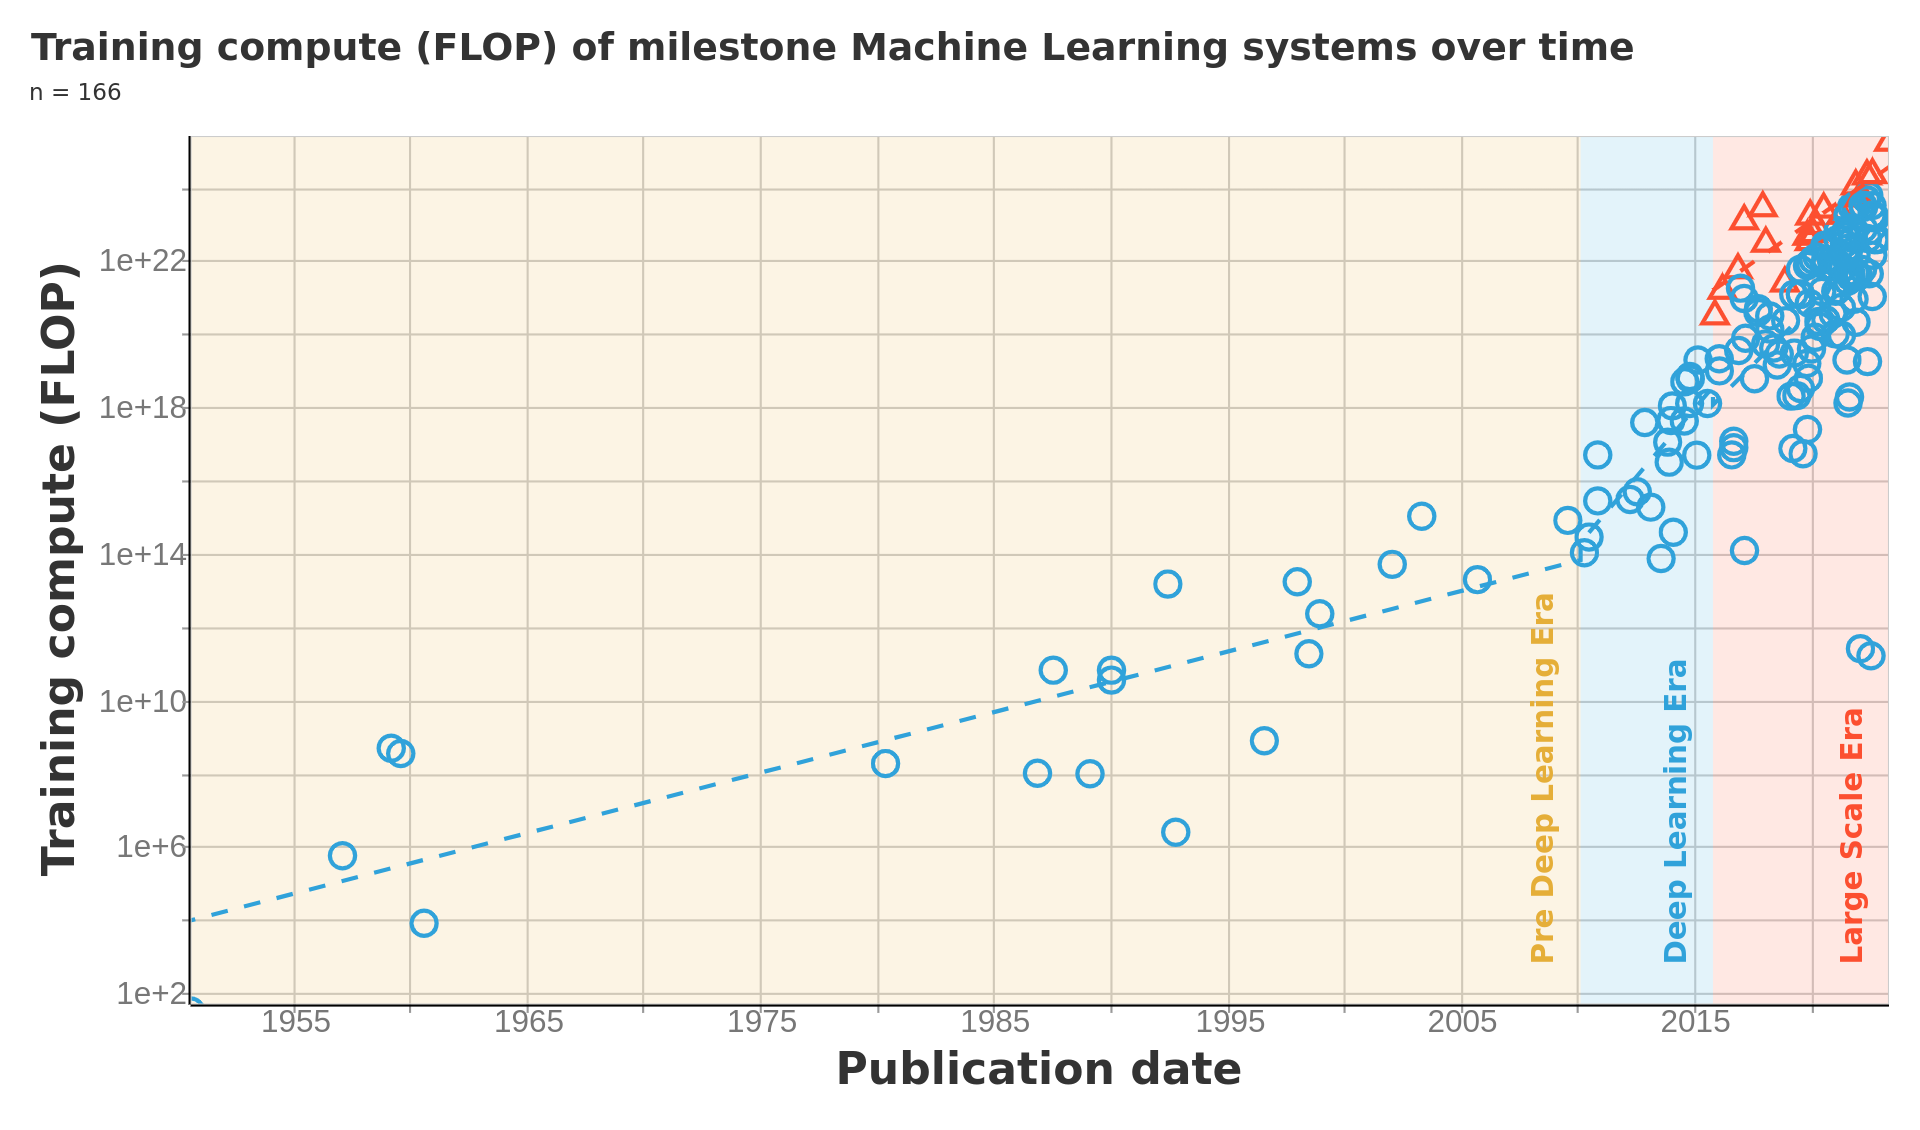
\includegraphics[width=0.8\textwidth]{figures/compute-trends.png}
    \caption{Compute trends are slower than previously reported}
    \label{fig:enter-label}
\end{figure}

Y las puedes citar siempre usando \ref{fig:enter-label}.

En primer lugar, las figuras juegan un papel crucial en la presentación de resultados, gráficos y diagramas. LaTeX permite incorporar imágenes en varios formatos, como PNG, JPEG o PDF. Al utilizar el entorno "figure", es posible agregar títulos, etiquetas y referencias cruzadas a las figuras para hacer referencia a ellas en el texto. La posibilidad de ajustar el tamaño, ubicación y alineación de las figuras permite una presentación visualmente atractiva y coherente.

Las tablas también son elementos esenciales en la presentación de datos tabulados. Con LaTeX, es posible crear tablas personalizadas utilizando el entorno "tabular". Se pueden definir diferentes formatos de celdas, alinear el contenido y agregar líneas horizontales y verticales para mejorar la legibilidad. Además, LaTeX permite etiquetar y referenciar tablas, lo que facilita la incorporación de análisis y discusiones específicas en el texto.

Mi recomendación es usar esta herramienta: \url{https://www.tablesgenerator.com/}. Se pueden subir las talas desde un excel, o llenarlas en linea y luego obtener el código para ponerlas aquí, es más sencillo, en latex escribir tablas puede ser un poco engorroso. Este es un ejemplo:

\begin{table}[htb]
\caption{Compute trends are slower than previously reported}
\label{tab:enter-label}
\centering
 \begin{tabular}{cccc} 
 \hline
 Col1 & Col2 & Col2 & Col3 \\ [0.5ex] 
 \hline
 1 & 6 & 87837 & 787 \\ 
 2 & 7 & 78 & 5415 \\
 3 & 545 & 778 & 7507 \\
 4 & 545 & 18744 & 7560 \\
 5 & 88 & 788 & 6344 \\
 \hline
 \end{tabular}
\end{table}

Otro aspecto importante son las ecuaciones matemáticas, especialmente en documentos académicos y científicos. LaTeX es conocido por su capacidad para producir ecuaciones de alta calidad y con una presentación profesional. Utilizando el modo matemático, se pueden crear ecuaciones simples o complejas mediante comandos y símbolos intuitivos. La numeración automática de ecuaciones permite hacer referencia a ellas fácilmente en el texto, garantizando una coherencia y claridad en la exposición de la información.

\begin{equation}
    E=Mc^2+\sqrt{\frac{1-\gamma}{\gamma_0}}m_Cv^2,
\end{equation}

LaTeX ofrece numerosas herramientas y paquetes que simplifican la inserción y gestión de figuras, tablas y ecuaciones. Por ejemplo, el paquete "graphicx" permite una manipulación flexible de imágenes, mientras que "booktabs" proporciona un formato de tabla profesional con líneas horizontales mejoradas. Además, para ecuaciones más avanzadas, el paquete "amsmath" ofrece una amplia gama de comandos matemáticos adicionales.

En conclusión, el uso adecuado de figuras, tablas y ecuaciones en documentos LaTeX mejora significativamente la presentación y comprensión del contenido. La capacidad para referenciar y organizar estos elementos gráficos brinda coherencia y facilita la lectura del documento. Con las herramientas y paquetes disponibles, LaTeX se convierte en una opción poderosa y versátil para aquellos que buscan producir documentos académicos, informes técnicos o trabajos científicos de alta calidad.